\chapter{OFFIXE}
\section{KD-82MS (Z171)}\index{OFFIXE!Z171}
Calcolatrice prodotta in Cina, probabile clone Casio FX-82MS\index{Casio!FX82MS}
\subsection{Test interno}
Il test\[\arcsin(\arccos(\arctan(\tan(\cos(\sin(9))))))=9\] ha come risulta dalla tabella~\vref{tab:OFFIXEKD82MS}. 
\subsection{PCB}
Sigla PCB:AL-1182
\subsection{Modi funzionamento}
La calcolatrice ha tre modi di funzionamento, calcoli aritmetici di base, deviazione standard, calcoli di regressione
\subsection{Formati visualizzazione}
Premere tasto \tastomode finché si ottiene la schermata
\begin{center}
	\CASIOmodediplayexp
	
\end{center}
\begin{description}
	\item[\tasto{1} FIX]Numero cifre decimali
	\item[\tasto{2} SCI]Numero cifre significative
	\item[\tasto{1} NORM]Formato di visualizzazione decimale
\end{description}
\subsection{Angoli}
Premere tasto \tastomode finché si ottiene la schermata
\begin{center}
	\CASIOmodediplayang
	
\end{center}
\begin{description}
	\item[\tasto{1} Deg]Gradi
	\item[\tasto{2} Rad]Radianti
	\item[\tasto{1} Gra]Gradi Centesimali
\end{description}
\begin{table}
	\centering
		\begin{tabular}{lll}
		\toprule
		\multicolumn{1}{c}{Modello}&\multicolumn{1}{c}{Risultato}&\multicolumn{1}{c}{Errore}\\
		\midrule
		OFFIXE KD-82MS(Z171)&\num{8.9999999998}&\num{1.921103e-9}\\
		\bottomrule
	\end{tabular} 
	\caption{OFFIXE KD-82MS (Z171)}
	\label{tab:OFFIXEKD82MS}
\end{table}
\begin{table}\centering
	\begin{tabular}{ccc}
	\toprule
	MODO	&TASTI  &  DISPLAY\\ 
		\midrule 
	Calcoli aritmetici di base	& \tastomode\tasto{1} & COMP \\ 
		\midrule 
	Deviazione standard	&\tastomode\tasto{2}  & SD \\ 
		\midrule 
	Calcoli di regressione	&\tastomode\tasto{3}  & REG  \\ 
		\bottomrule
	\end{tabular} 
		\caption{Modi: OFFIXE KD-82MS (Z171)}
	\label{tab:OFFIXEKD82MSModi}
\end{table}
\begin{figure}
	\begin{subfigure}[b]{.5\linewidth}
	\centering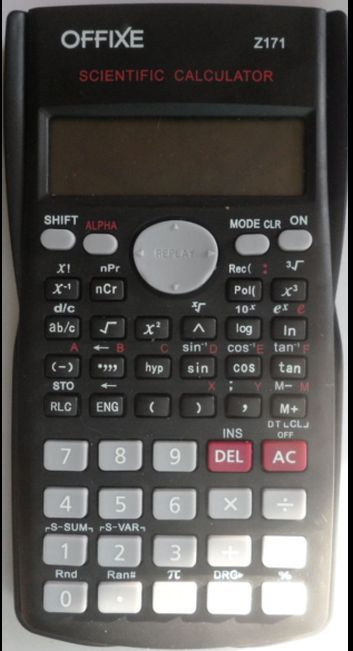
\includegraphics{offixe/SAM_3719}%
		\caption{Fronte}\label{fig:OFFIXEfront}
	\end{subfigure}%
	\begin{subfigure}[b]{.5\linewidth}
   \centering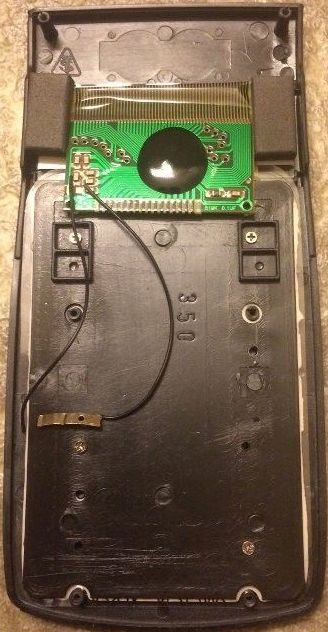
\includegraphics{offixe/7019561509344433257}%
		\caption{PCB}\label{fig:OFFIXEPCB}
	\end{subfigure}
	\caption{OFFIXE KD-82MS (Z171)}\label{fig:OFFIXEKD82MS}
\end{figure}
